\documentclass[11pt,a4paper]{article}

% ==============================================================================
% EXPERIMENT 02: PRINTABLE SOURCE CODE & OUTPUT (EXACT SINGLE 1-PAGE DOCUMENT)
% Formatted with 1.0-inch lateral margins, large readable fonts, and tight top/bottom margins.
% ==============================================================================
\usepackage[utf8]{inputenc}
\usepackage[T1]{fontenc}
\usepackage{lmodern}
\usepackage[left=1.0in, right=1.0in, top=0.35in, bottom=0.35in]{geometry}
\usepackage{amsmath,amssymb}
\usepackage{listings}
\usepackage{tikz}
\usetikzlibrary{arrows.meta,positioning,calc}
\usepackage{booktabs}
\usepackage{tabularx}
\usepackage{titlesec}
\usepackage{caption}
\usepackage{microtype}
\usepackage{float}

% Disable all running headers, footers, and page numbers for clean print & paste
\pagestyle{empty}
\setlength{\parindent}{0pt}

% Section Titles Formatting (Enlarged)
\titleformat{\section}
  {\normalfont\large\bfseries\raggedright}{\thesection}{0.6em}{}[\titlerule]

\titlespacing*{\section}{0pt}{6pt}{3pt}

% Code Listing Styling (Strict Monochrome with Enlarged Font for High-Contrast Print)
\lstdefinestyle{bwArduino}{
    language=C++,
    basicstyle=\ttfamily\footnotesize,
    keywordstyle=\bfseries,
    commentstyle=\itshape,
    stringstyle=\ttfamily,
    numbers=left,
    numberstyle=\tiny,
    numbersep=6pt,
    stepnumber=1,
    breaklines=true,
    breakatwhitespace=true,
    frame=single,
    rulecolor=\color{black},
    tabsize=2,
    showstringspaces=false,
    columns=fullflexible,
    keepspaces=true,
    lineskip=0.4pt,
    aboveskip=2pt,
    belowskip=2pt
}

\captionsetup{font=small,labelfont=bf,skip=2pt}

\begin{document}

% ==============================================================================
% DOCUMENT HEADER
% ==============================================================================
\begin{center}
    {\Large\bfseries Experiment 02: Interfacing Dual Alternating LEDs with Arduino UNO}\\[0.10cm]
    {\normalsize\textbf{GPIO Digital Output Control --- Program Source Code \& Circuit State Output}}
\end{center}
\vspace{-0.20cm}
\rule{\textwidth}{0.9pt}
\vspace{0.06cm}

% ==============================================================================
% 1. PROGRAM SOURCE CODE
% ==============================================================================
\section*{1. Arduino C++ Source Code}

\begin{lstlisting}[style=bwArduino, title={\textbf{Listing 2.1: Microcontroller Firmware for Periodic Anti-Phase LED Blinking.}}]
/*
 * Experiment 02: Dual Alternating LED Interfacing with Arduino UNO
 * Hardware Pin Connections:
 *   - Arduino Digital Pin 8 -> Green LED Anode (via 1 kOhm Resistor R1)
 *   - Arduino Digital Pin 7 -> Red LED Anode   (via 1 kOhm Resistor R2)
 *   - Common Ground (GND)   -> LED Cathodes
 * Switching Interval: 1000 ms (1.0 second periodic period)
 */
const int LED1_PIN = 8;    // Green LED Channel (Digital Pin D8)
const int LED2_PIN = 7;    // Red LED Channel   (Digital Pin D7)
const unsigned long BLINK_INTERVAL = 1000; // Period: 1000 ms (1.0 s)

void setup() {
  pinMode(LED1_PIN, OUTPUT); // Configure D8 as push-pull output driver
  pinMode(LED2_PIN, OUTPUT); // Configure D7 as push-pull output driver
  digitalWrite(LED1_PIN, LOW); // Initialize D8 LOW
  digitalWrite(LED2_PIN, LOW); // Initialize D7 LOW
}

void loop() {
  // Phase 1: LED1 ON (Active-HIGH 5V), LED2 OFF (Active-LOW 0V)
  digitalWrite(LED1_PIN, HIGH);
  digitalWrite(LED2_PIN, LOW);
  delay(BLINK_INTERVAL);
  // Phase 2: LED1 OFF (Active-LOW 0V), LED2 ON (Active-HIGH 5V)
  digitalWrite(LED1_PIN, LOW);
  digitalWrite(LED2_PIN, HIGH);
  delay(BLINK_INTERVAL);
}
\end{lstlisting}

\vspace{0.06cm}

% ==============================================================================
% 2. EXPERIMENTAL OUTPUT & LOGIC WAVEFORMS (SERIAL: 2.A -> 2.B)
% ==============================================================================
\section*{2. Experimental Output, Logic Timing \& Truth Table}

\noindent
\textbf{A. Circuit State Truth Table \& Switching Log:}\par\vspace{0.06cm}
{\footnotesize
\setlength{\tabcolsep}{5pt}
\renewcommand{\arraystretch}{1.18}
\begin{tabularx}{\textwidth}{|c|c|c|X|}
\hline
\textbf{Interval} & \textbf{Pin 8 Output} & \textbf{Pin 7 Output} & \textbf{Observed Hardware State} \\
\hline
$0 - 1\,\text{s}$ & HIGH ($5\,\text{V}$) & LOW ($0\,\text{V}$) & \textbf{$\text{LED}_1$ ON}, $\text{LED}_2$ OFF ($I_{F1} \approx 3\,\text{mA}$, Green LED ON) \\
$1 - 2\,\text{s}$ & LOW ($0\,\text{V}$) & HIGH ($5\,\text{V}$) & $\text{LED}_1$ OFF, \textbf{$\text{LED}_2$ ON} ($I_{F2} \approx 3\,\text{mA}$, Red LED ON) \\
$2 - 3\,\text{s}$ & HIGH ($5\,\text{V}$) & LOW ($0\,\text{V}$) & \textbf{$\text{LED}_1$ ON}, $\text{LED}_2$ OFF (Periodic Alternation) \\
$3 - 4\,\text{s}$ & LOW ($0\,\text{V}$) & HIGH ($5\,\text{V}$) & $\text{LED}_1$ OFF, \textbf{$\text{LED}_2$ ON} (Periodic Alternation) \\
\hline
\end{tabularx}
}

\vspace{0.20cm}

\noindent
\textbf{B. Digital Timing Waveforms (Anti-Phase Switching, $T = 1.0\,\text{s}$):}\par\vspace{0.05cm}
{\centering
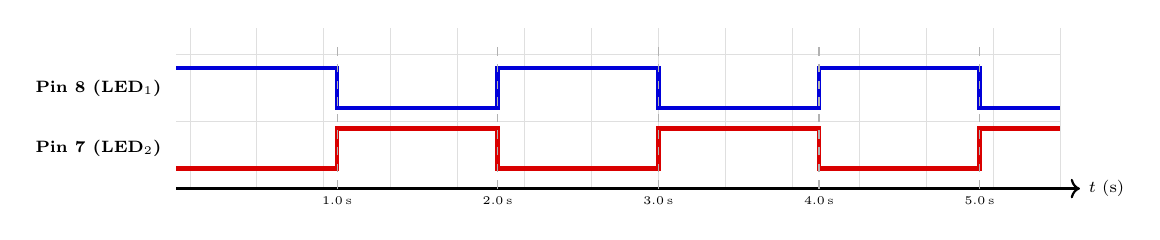
\begin{tikzpicture}[scale=0.85, every node/.style={transform shape}]
    \draw[step=1.0cm,gray!25,very thin] (1.8,0) grid (15.0,2.4);
    \draw[thick,->] (1.8,0) -- (15.3,0) node[right, font=\scriptsize] {$t$ (s)};
    
    % Pin 8 (LED1)
    \draw[ultra thick, blue!85!black] (1.8,1.8) -- (4.2,1.8) -- (4.2,1.2) -- (6.6,1.2) -- (6.6,1.8) -- (9.0,1.8) -- (9.0,1.2) -- (11.4,1.2) -- (11.4,1.8) -- (13.8,1.8) -- (13.8,1.2) -- (15.0,1.2);
    \node[left, font=\scriptsize\bfseries] at (1.7,1.5) {Pin 8 ($\text{LED}_1$)};

    % Pin 7 (LED2)
    \draw[ultra thick, red!85!black] (1.8,0.3) -- (4.2,0.3) -- (4.2,0.9) -- (6.6,0.9) -- (6.6,0.3) -- (9.0,0.3) -- (9.0,0.9) -- (11.4,0.9) -- (11.4,0.3) -- (13.8,0.3) -- (13.8,0.9) -- (15.0,0.9);
    \node[left, font=\scriptsize\bfseries] at (1.7,0.6) {Pin 7 ($\text{LED}_2$)};
    
    \foreach \x/\t in {4.2/1.0\,s, 6.6/2.0\,s, 9.0/3.0\,s, 11.4/4.0\,s, 13.8/5.0\,s} {
        \draw[dashed, gray!60] (\x,0) -- (\x,2.2);
        \node[below, font=\tiny] at (\x,0) {\t};
    }
\end{tikzpicture}\par\vspace{0.05cm}
{\small\textbf{Figure 2.1:} Digital logic anti-phase switching waveforms for complementary LED driving.}\par}

\end{document}
